\documentclass{article}
\usepackage{graphicx}
\usepackage[strings]{underscore}
\usepackage{url}
\usepackage[margin=2cm]{geometry}

\usepackage{titlesec}
\newcommand{\sectionbreak}{\clearpage}

\title{Large Dynamic Voxel Scenes using Sparse Voxel Octrees}
\author{Nicolas Fedor, 6683787}
\date{May 2025}

\begin{document}
\maketitle

\section{Introduction}
Voxel rendering has become an essential technique in computer graphics, enabling the representation and visualization of 3D environments through volumetric data. Unlike traditional polygon-based methods that rely on triangles and surface meshes, voxel rendering represents scenes as a grid of volumetric elements (voxels), which allows for detailed depictions of complex structures such as terrains, clouds, or medical imaging data. This approach offers several advantages, particularly in handling volumetric and procedural data, but also poses significant challenges, including high memory consumption and computational demands.

Several data compression techniques have been developed to address these challenges, such as Sparse Voxel Octrees (SVOs) and Sparse Voxel Directed Acyclic Graphs (SVDAGs). These methods aim to reduce memory usage by representing voxel data in a hierarchical, sparse format, allowing for efficient storage and rendering of large voxel grids. However, dynamic scenes present additional challenges, as updating the highly compressed voxel data structure in real-time can be computationally expensive.

This project will explore the usage of an SVO for rendering a large world and the challenges of dynamic voxel data. By optimizing the construction of the SVO, and creating a clear separation of static and dynamic voxel data, this work aims to achieve real-time rendering of dynamic voxel worlds with minimal memory footprint; such that it could be run on low-end hardware.

\subsection{Aims and Objectives}
The aim of this project is to develop a dynamic voxel rendering system using an SVO data structure. There are two main objectives:

\begin{itemize}
    \item Design and implement an SVO data structure for representing voxel data.
    \item Optimize SVO updates for real-time rendering of dynamic voxel worlds.
\end{itemize}

\subsubsection{Sparse Voxel Octree Data Structure}
Voxel data can take up a large amount of memory, especially for high-resolution grids. The SVO data structure aims to compress the voxel data by representing the volume as a tree of nodes, where each node contains either a single voxel or a pointer to a child node. This hierarchical representation allows for efficient storage and traversal of the voxel data, reducing the memory footprint and improving rendering performance. The objective is to design and implement an SVO data structure that can efficiently store and render large voxel worlds, using previous works as a reference~\cite{Laine_Karras_2010}.

\begin{itemize}
    \item Design and implement an SVO data structure for representing voxel data.
    \item Optimize SVO construction and traversal for real-time rendering.
    \item Achieve a minimal memory footprint for rendering large voxel worlds.
\end{itemize}

\subsubsection{Dynamic Voxel Data}
Dynamic voxel data presents additional challenges, as updating the voxel grid in real-time can be computationally expensive. The objective is to optimize the SVO updates for dynamic voxel worlds, by separating static and dynamic voxel data, and efficiently updating the SVO structure to reflect changes in the voxel grid. This will involve developing techniques for efficiently updating the SVO while maintaining real-time rendering performance, based on previous works~\cite{Crassin_2012}.

\section{Literature Review}
This chapter will provide an overview of the existing techniques for rendering voxel data, including traditional mesh-based methods and recent advances using ray tracing and sparse voxel representations.

\subsection{Mesh-based Rendering}
Mesh-based rendering is the most common technique for representing 3D objects in computer graphics. It involves defining the surface of an object using a collection of polygons, typically triangles, which are then rendered using the GPU's rasterization pipeline. This is a well-established approach, that is the default method for rendering 3D graphics in most applications.

Volumetric voxel data can be converted to a mesh representation using techniques such as Marching Cubes~\cite{Amran_1998}, which extract the surface of the volume by sampling the voxel data; or another simpler, popular, approach is to use greedy meshing~\cite{mikolalysenko_2012}, which relies on creating a mesh by merging adjacent voxels with the same material into a single quad face in the mesh. These approaches allow for storing voxel data uncompressed and so dynamic updates to voxel data are quick. However, the generation of the mesh becomes a bottleneck as the resolution of the voxel data increases.

\subsection{Ray Marching}
Ray marching, a specialized form of ray tracing, is another technique for rendering voxel data. It involves casting a ray through a 3D grid of voxels and sampling the voxel data along the ray to determine the color and opacity of the volume at each point. Ray marching can be implemented on the GPU using compute shaders, avoiding the creation of a mesh, instead the GPU can operate directly on the voxel data, which can be stored in a compressed format.

\subsubsection{Digital Differential Analysis (DDA)}
A common technique for ray marching is Digital Differential Analysis (DDA), which involves stepping through the voxel grid along the ray using fixed-size increments or steps calculated based on the ray direction. At each step, the voxel data is sampled to determine the color and opacity of the volume, which is accumulated along the ray to produce the final image. DDA is a simple and efficient method for ray marching~\cite{Amanatides_Woo_1987}, but intersection testing a ray is an expensive operation and so limiting the number of intersection tests a ray tracer must perform is important for real-time rendering.

\subsection{Data Compression}
Compressing a voxel grid is essential for rendering large voxel worlds efficiently using ray marching as the number of intersection tests has a large impact on ray tracing performance, in ray tracing Binary Space Partitioning is a way of improving ray tracing performance~\cite{Ize_2009}.

Sparse Voxel Octrees (SVOs) emerged as a popular solution to compressing voxel data. SVOs are a hierarchical data structure that represents a voxel grid as a tree of nodes, where each node contains either a single voxel or a pointer to a child node; the aim here is to reduce the memory usage by storing only the voxels that are necessary to represent the volume i.e. by collapsing "chunks" of similar voxels into a single node. An example of an SVO is shown in Figure~\ref{fig:svo}.

\begin{figure}[thp]
    \begin{center}
        \scalebox{0.5}{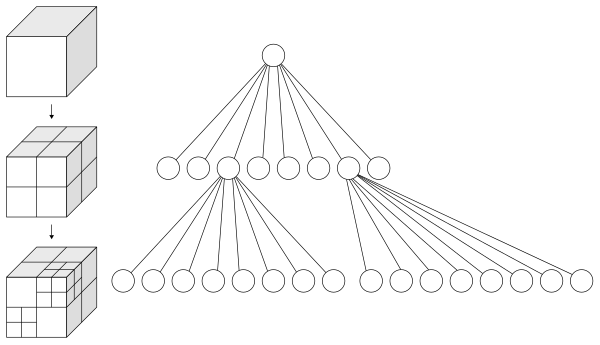
\includegraphics[width=0.8\textwidth]{figures/octree.png}}
    \end{center}
    \caption{Illustration of an Octree representation of a voxel grid. Source: Wikipedia}
    \label{fig:svo}
\end{figure}

Additional techniques for compression voxel data like Sparse Voxel Directed Acyclic Graphs (SVDAGs) have been proposed and these are even better suited to storing large, high-resolution voxel worlds~\cite{Kampe_Sintorn_Assarsson}. SVDAGs are similar to SVOs but allow for more efficient compression by sharing identical subtrees between nodes, as shown in Figure~\ref{fig:svdag}.

\subsection{Dynamic Voxel Data}
Minecraft is a voxel-based video game that makes use of mesh-based rendering~\label{Mesh-based Rendering} to render its voxel world. The game supports dymanic updates to the voxel world by separating the world into smaller chunks, which can be updated independently of each other. This allows for efficient updates to the voxel data, as only the affected chunks need to be modified, and the rest of the world can remain static.

Another approach for voxel modification is by storing an "overlay" of the modified voxels on top of the static voxel data. In ray marching, initial rays are cast through the static voxel data, and then the overlay can be checked for any modifications to the voxel data. This approach allows for dynamic updates to the voxel world without modifying the underlying voxel data. Since SVOs are hierachical in their nature, it is possible to store the overlay as a separate SVO, which can be merged with the static SVO~\cite{Douglas_2022} at a later stage.

\section{Technical Overview}
This chapter will provide a technical overview of the proposed dynamic voxel rendering system.

\subsection{Voxel Data Representation}
The voxel world will be split into chunks, where each chunk will represent a fixed size voxel grid; each chunk will store its own voxel data as an SVO.

\subsubsection{Sparse Voxel Octree}

\subsection{Graphical Pipeline}

\subsection{Dynamic Voxel Updates}

\section{Workplan}
The following work plan is what I will be using for the project is shown in Figure.

\bibliographystyle{IEEEtran}
\bibliography{references}

\end{document}
